\documentclass[11pt]{article}
\usepackage{graphicx}
\graphicspath{ {./images/} }

\usepackage{algorithm}
\usepackage{algpseudocode}
\usepackage{hyperref}

\usepackage{sectsty}
\usepackage{graphicx}
\usepackage[font=small,labelfont=bf]{caption} % Required for specifying captions to tables and figures

% Margins
\topmargin=-0.45in
\evensidemargin=0in
\oddsidemargin=0in
\textwidth=6.5in
\textheight=9.0in
\headsep=0.25in

\title{ %

\includegraphics[width=0.4\textwidth]{UniCT-Logo-Nero}~\\
A solution for MWVC using Iterated Local Search \\ 
\large Laboratorio Intelligenza Artificiale (LM-18) \\ Università degli Studi di Catania - A.A 2021/2022 \\
}
\author{ Danilo Leocata \\ Docente: Mario Pavone}
\date{\today}

\begin{document}

\maketitle	
\pagebreak

% Optional TOC
% \tableofcontents
% \pagebreak

%--Paper--

\section{Introduzione}

Si propone una soluzione per il Weight Vertex Cover problem utilizzando l'Iterated Local Search: l'obbiettivo proposto è trovare la migliore soluzione, data un istanza, con il minimo numero di iterazioni. I
Il codice è stato interamente in Java senza utilizzare librerie esterne eccetto \verb|matplotlib4j| per la generazione dei grafici di convergenza e \verb|CSVWriter| per la generazione del \verb|.csv| dei benchmarks.

Il codice è interamente disponibile al seguente repository GitHub \href{https://github.com/khalld/mwvc-using-ils-java}{https://github.com/khalld/mwvc-using-ils-java}, nel quale sono stati caricati i risultati di benchmark e parte dei grafici di convergenza realizzati.

Prima di procedere con l'implementazione e la scelta dell'algoritmo, sono state consultate e prese in considerazioni varie pubblicazioni riguardanti la soluzione del problema (indicate a fine relazione). È stata trovata sin da subito interessante implementare una soluzione utilizzando l'Iterated Local Search rispetto all'algoritmo genetico con il quale è computazionalmente più oneroso trovare una buona soluzione iniziale.
Se si riuscisse a trovare una buona soluzione iniziale ed implementando un operatore di perturbazione sarebbe più semplice ottenere soluzioni vicine da valutare.

\pagebreak

\section{Generazione della soluzione iniziale}

Banalmente è stato trovato opportuno implementare un algoritmo greedy per costruire la soluzione iniziale. Sono stati effettuati dei test in cui il punto di partenza è la soluzione \textit{peggiore} (che contiene tutti i nodi dell'istanza) le cui performance sono sempre state peggiori rispetto all'algoritmo greedy

\begin{algorithm}
    \caption{\texttt{GetInitialSolution}}
    \begin{algorithmic}
        \Require {\texttt{graph, allVertex}}
        
        \State{\texttt{totalWeight = 0}}
        \State{\texttt{selectedVertex = initialize empty list of vertex}}
        \State{\texttt{selectedEdges = initialize empty list of edges}}

        \For{\texttt{edge in allEdges}}
        \State \texttt{get source and destination of current edge}
        \State \texttt{if is already explored, skip}

        \If{\texttt{sourceVertexWeight < destVertexWeight}}
            \State\texttt {set sourceVertex explored}
            \State\texttt{totalWeight+= sourceVertexWeight}
            \State{\texttt{add sourceVertex to selectedVertex}}
            \State{\texttt{add current edge to selectedEdges}}

        \Else{\texttt{}}

        \State\texttt {set destVertex explored}
        \State\texttt{totalWeight+= destVertexWeight}
        \State{\texttt{add destVertex to selectedVertex}}
        \State{\texttt{add current edge to selectedEdges}}


        \EndIf{}
        \EndFor
        

    \Return { \texttt{Initial Solution}}
    \end{algorithmic}
    \end{algorithm}


\pagebreak

\section{Validità della soluzione}

La soluzione è da considerarsi completa e valida se tutti gli archi del grafo sono esplorati: di conseguenza sarà necessario controllare la validità della soluzione dopo la rimozione di un nodo.
Una generica soluzione viene dunque validata scorrendo la lista di adiacenza di tutti i nodi selezionati: se dunque non saranno presenti tutti gli archi del grafo allora sarà considerata non valida.

\section{Operatore di perturbazione}

L'idea generale della perturbazione è quella di modificare i parametri ad ogni iterazione applicando una perturbazione sui nodi selezionati dalla soluzione.
È stato inoltre già dimostrato da una delle referenze citate che una perturbazione troppo forte potrebbe portare allo stallo dell'ottimo locale: di è conseguenza in una
prima fase si è deciso di implementare la seguente:

Un buon algoritmo deve evitare di far cadere sempre nello stesso minimo locale, in generale:

\begin{algorithm}
\caption{\texttt{WeakPerturbation}}
\begin{algorithmic}
\Require{ \texttt{Solution, availableVertex} }

\If{\texttt{ there aren't nodes not selected }}
\State\texttt{remove random vertex from already seleceted}

\Else{}
\State\texttt{remove random vertex from already seleceted}
\State\texttt{add random vertex from list of not seleceted}

\EndIf{}

\end{algorithmic}
\end{algorithm}

Tra le migliorie che la perturbazione potrebbe apportare alla soluzione vi è:
\begin{itemize}
\item{l'eliminazione automaticamente di cicli se questa contiene dei nodi ridondanti;}
\item{potrebbe rendere la soluzione non completa: di conseguenza applicando nuovamente la LocalSearch è possibile trovare un nodo candidato migliore rispetto a quello rimosso.}
\end{itemize}

Tuttavia è stato notato, durante fasi di sviluppo, che questo operatore tendeva a perdere efficacia in quanto tendeva a bloccare la soluzione sull'ottimo locale.
Di conseguenza, è trovato opportuno introdurre un parametro $\epsilon$ ed una variante della \texttt{Weakperturbation}:

\begin{algorithm}
    \caption{\texttt{SecondChoicePerturbation}}
    \begin{algorithmic}
    \Require{ \texttt{Solution, availableVertex} }
    \State\texttt{remove random vertex from already seleceted}    
\end{algorithmic}
\end{algorithm}

Il parametro $\epsilon$ rappresenta banalmente la percentuale di \textit{risparmio} sul costo tra la soluzione corrente e quella peggiore.
La \texttt{SecondChoicePerturbation} verrà utilizzata solo quando $\epsilon$ sarà maggiore di \verb|25|: in questo modo la perturbazione non contribuirà al \textit{lock} sull'ottimo locale.

\pagebreak


\section{Criterio di accettazione}

Per evitare che il criterio accetti solo soluzioni migliori rispetto alla precedente è stata introdotta una componente randomica per accettare anche soluzioni \textit{non migliori}.

\section{Local Search e criterio di selezione del nodo migliore}

\begin{algorithm}
\caption{LocalSearch}
\begin{algorithmic}
\Require{ \texttt{Solution}}

\If{
    given solution has unreached nodes
}   
    \State\texttt{evaluate if swapping some nodes brings benefits to the solution }
    \State\texttt{increment counter for every evalutation}
\Else{}
\State\texttt{evaluate if removing some nodes brings benefits to the solution }
    \State\texttt{increment counter for every evalutation}
\EndIf{}

\State{\texttt{update solution}}

\State \Return updated solution
\end{algorithmic}
\end{algorithm}

\pagebreak

\section{Criterio di accettazione}

L'utilizzo del term memory permette di 'accettare' soluzioni peggiori rispetto ad altre e continuare la ricerca senza perder traccia di tutte le soluzioni trovate.
In sintesi, se la soluzione perturbata è simile alla corrente il criterio di accettazione può ripescare, randomicamente una delle soluzioni presenti nel \verb|term-memory| e continuare la ricerca.
È stato introdotto inolte un \verb|lockCounter| per evitare che la soluzione rimanga bloccata su un ottimo locale.


\begin{algorithm}
\caption{\texttt{Acceptance criteria}}
\begin{algorithmic}
    \Require \texttt{prev solution, new solution, term memory, lockCounter}
    \If{
        \State\texttt{cost old solution > cost new solution }
        \Return\texttt{new solution}
    }
    \Else{
        \State\texttt{if lockCounter = to maxValue}
        \State\Return\texttt{random solution from term-memory}
    }

    \EndIf{}
    
    \State \Return \texttt{random choice between (perturbed solution, current solution)}
\end{algorithmic}
\end{algorithm}

Tuttavia nella pratica questa ricerca non ha sempre portato a buoni risultati, di conseguenza è stato disabilitato.

\pagebreak

\section{Benchmarks e conclusione}

È stato implementato uno script che permette di salvare i benchmark le soluzioni ottenute dalle istanze su  file \verb|.csv|, oltre alla creazione dei grafici di convergenza.
I grafici importati ed le tabelle fanno riferimento alle run con \verb|WeakPerturbation|. n certi casi, si rimane bloccati su un ottimo locale per molto tempo, fino a quando una soluzione perturbata non ottimale fa da punto di partenza per trovare una soluzione migliore.
Si nota inoltre che un numero maggiore di nodi o archi non implica necessariamente un numero maggiore di valutazioni: anche grafi con lo stesso numero di nodi e archi hanno valori molto contrastanti, probabilmente perché il problema dipende molto dal peso dei nodi e dalla topologia del grafo.

\begin{center}
\begin{minipage}{0.48\linewidth}
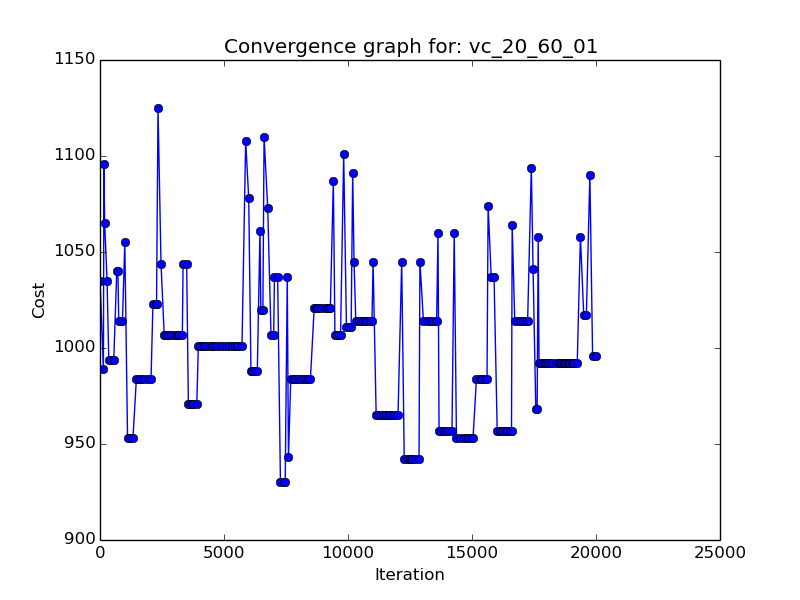
\includegraphics[width=\linewidth]{cg_1.png}
\end{minipage}%
\begin{minipage}{0.49\linewidth}
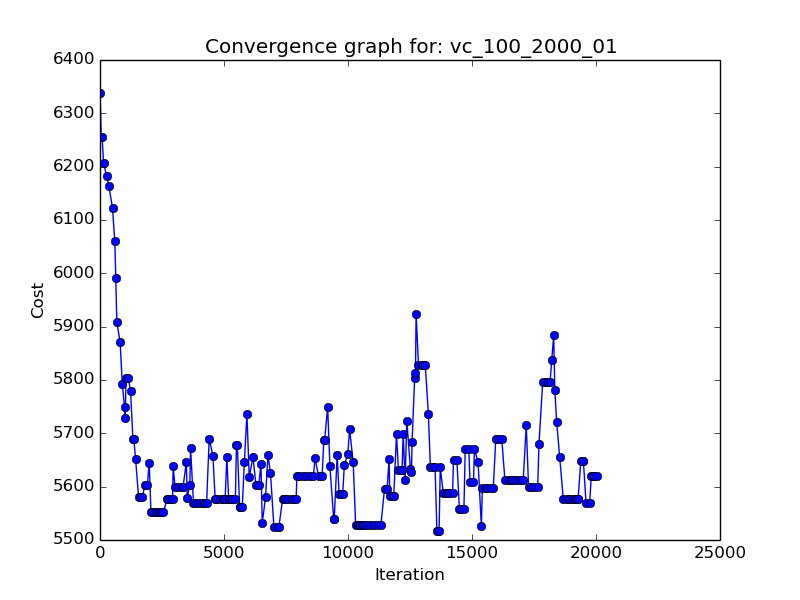
\includegraphics[width=\linewidth]{cg_2.png}
\end{minipage}
\begin{minipage}{0.49\linewidth}
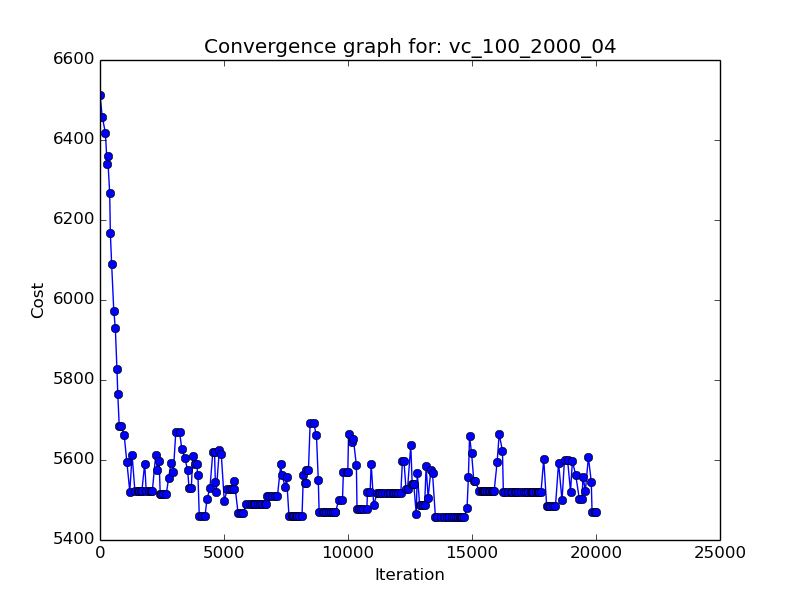
\includegraphics[width=\linewidth]{cg_3.png}
\end{minipage}
\begin{minipage}{0.49\linewidth}
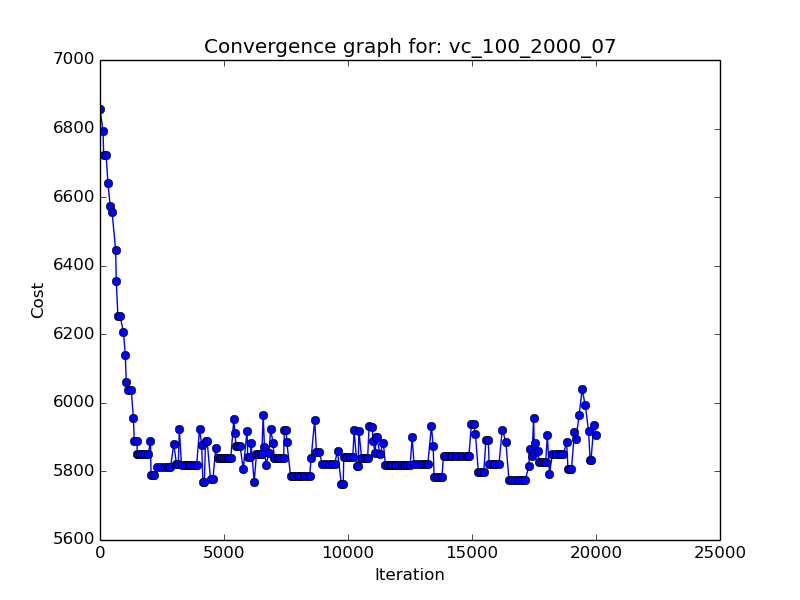
\includegraphics[width=\linewidth]{cg_4.png}
\end{minipage}
\captionof{figure}{Sample grafici di convergenza}
\end{center}

\pagebreak

\begin{table}[!ht]
    \centering
    \begin{tabular}{|l|l|l|l|}
    \hline
        instance & best solution & best solution iter & elapsed ms \\ \hline

        vc\_20\_120\_01 & 1253 & 77 & 99 \\ \hline
        vc\_20\_120\_02 & 1348 & 191 & 94 \\ \hline
        vc\_20\_120\_03 & 1319 & 58 & 92 \\ \hline
        vc\_20\_120\_04 & 1414 & 1179 & 99 \\ \hline
        vc\_20\_120\_05 & 1293 & 761 & 92 \\ \hline
        vc\_20\_120\_06 & 1271 & 77 & 102 \\ \hline
        vc\_20\_120\_07 & 1265 & 1806 & 98 \\ \hline
        vc\_20\_120\_08 & 1520 & 1654 & 98 \\ \hline
        vc\_20\_120\_09 & 1587 & 229 & 97 \\ \hline
        vc\_20\_120\_10 & 1452 & 381 & 95 \\ \hline
        vc\_20\_60\_01 & 1105 & 405 & 33 \\ \hline
        vc\_20\_60\_02 & 1585 & 476 & 37 \\ \hline
        vc\_20\_60\_03 & 1313 & 58 & 34 \\ \hline
        vc\_20\_60\_04 & 1177 & 115 & 37 \\ \hline
        vc\_20\_60\_05 & 1352 & 324 & 37 \\ \hline
        vc\_20\_60\_06 & 1426 & 343 & 33 \\ \hline
        vc\_20\_60\_07 & 1573 & 210 & 36 \\ \hline
        vc\_20\_60\_08 & 1526 & 39 & 36 \\ \hline
        vc\_20\_60\_09 & 1595 & 324 & 36 \\ \hline
        vc\_20\_60\_10 & 1416 & 552 & 35 \\ \hline
        vc\_25\_150\_01 & 1785 & 265 & 108 \\ \hline
        vc\_25\_150\_02 & 1472 & 241 & 103 \\ \hline
        vc\_25\_150\_03 & 1658 & 20000 & 105 \\ \hline
        vc\_25\_150\_04 & 1923 & 97 & 103 \\ \hline
        vc\_25\_150\_05 & 1792 & 1849 & 114 \\ \hline
        vc\_25\_150\_06 & 1651 & 505 & 99 \\ \hline
        vc\_25\_150\_07 & 1977 & 841 & 104 \\ \hline
        vc\_25\_150\_08 & 1693 & 361 & 107 \\ \hline
        vc\_25\_150\_09 & 1739 & 841 & 111 \\ \hline
        vc\_25\_150\_10 & 1547 & 553 & 102 \\ \hline
        vc\_200\_750\_01 & 14160 & 1991 & 280 \\ \hline
        vc\_200\_750\_02 & 13384 & 399 & 201 \\ \hline
        vc\_200\_750\_03 & 14509 & 6767 & 297 \\ \hline
        vc\_200\_750\_04 & 13230 & 797 & 306 \\ \hline
        vc\_200\_750\_05 & 14495 & 399 & 211 \\ \hline
        vc\_200\_750\_06 & 13586 & 1792 & 325 \\ \hline
        vc\_200\_750\_07 & 13197 & 7762 & 286 \\ \hline
        vc\_200\_750\_08 & 13676 & 9155 & 298 \\ \hline
        vc\_200\_750\_09 & 13710 & 200 & 208 \\ \hline
        vc\_200\_750\_10 & 13794 & 399 & 211 \\ \hline
    \end{tabular}
\end{table}

\pagebreak

\begin{table}[!ht]
    \centering
    \begin{tabular}{|l|l|l|l|}
    \hline
        instance & best solution & best solution iter & elapsed ms \\ \hline

        
        vc\_100\_2000\_01 & 7027 & 1189 & 3158 \\ \hline
        vc\_100\_2000\_02 & 6853 & 20000 & 2970 \\ \hline
        vc\_100\_2000\_03 & 6680 & 20000 & 3032 \\ \hline
        vc\_100\_2000\_04 & 6890 & 6535 & 2984 \\ \hline
        vc\_100\_2000\_05 & 7236 & 8812 & 3093 \\ \hline
        vc\_100\_2000\_06 & 6876 & 2080 & 2873 \\ \hline
        vc\_100\_2000\_07 & 7322 & 4753 & 3103 \\ \hline
        vc\_100\_2000\_08 & 7163 & 1090 & 2930 \\ \hline
        vc\_100\_2000\_09 & 6829 & 793 & 3073 \\ \hline
        vc\_100\_2000\_10 & 7238 & 1882 & 2977 \\ \hline
        vc\_100\_500\_01 & 6739 & 5446 & 252 \\ \hline
        vc\_100\_500\_02 & 7205 & 496 & 225 \\ \hline
        vc\_100\_500\_03 & 6764 & 10331 & 220 \\ \hline
        vc\_100\_500\_04 & 6818 & 9802 & 242 \\ \hline
        vc\_100\_500\_05 & 7185 & 2278 & 254 \\ \hline
        vc\_100\_500\_06 & 7228 & 3961 & 237 \\ \hline
        vc\_100\_500\_07 & 6763 & 194 & 81 \\ \hline
        vc\_100\_500\_08 & 6788 & 397 & 250 \\ \hline
        vc\_100\_500\_09 & 6894 & 193 & 226 \\ \hline
        vc\_100\_500\_10 & 6670 & 2773 & 244 \\ \hline
        vc\_200\_3000\_01 & 13795 & 200 & 2648 \\ \hline
        vc\_200\_3000\_02 & 13790 & 20000 & 4038 \\ \hline
        vc\_200\_3000\_03 & 14245 & 8956 & 4144 \\ \hline
        vc\_200\_3000\_04 & 15082 & 598 & 2681 \\ \hline
        vc\_200\_3000\_05 & 14095 & 9354 & 4136 \\ \hline
        vc\_200\_3000\_06 & 13731 & 2588 & 4196 \\ \hline
        vc\_200\_3000\_07 & 14247 & 16717 & 4083 \\ \hline
        vc\_200\_3000\_08 & 14197 & 200 & 3903 \\ \hline
        vc\_200\_3000\_09 & 14294 & 19901 & 4141 \\ \hline
        vc\_200\_3000\_10 & 13907 & 4976 & 3982 \\ \hline
        vc\_800\_10000 & 56404 & 6393 & 52037 \\ \hline

    \end{tabular}
\end{table}

\pagebreak

Una delle difficoltà più grandi trovate durante l'implementazione è stato quello di determinare se i criteri di scelta fossero effettivamente robusti o no. Sarebbe interessante proseguire con lo studio del problema continuando sui seguenti punti:

\begin{itemize}
    \item{implementare altri criteri per la selezione del nodo;}
    \item{implementare altri criteri di accettazione;}
    \item{perfezionare l'algoritmo su istanze piccole;}
    \item{minimizzare il numero di valutazioni della fitness;}
\end{itemize}

\pagebreak

\begin{thebibliography}{6}

\bibitem{1} \href{https://www.researchgate.net/publication/242463011_An_Effective_Algorithm_for_Minimum_Weighted_Vertex_Cover_problem}{An Effective Algorithm for Minimum Weighted Vertex Cover Problem}
\bibitem{2} \href{https://www.cs.umd.edu/class/fall2018/cmsc858E/pdfs/651/vc.pdf} {Two approximation algorithm for Vertex Cover} 
\bibitem{3} \href{https://ieeexplore.ieee.org/abstract/document/7550782}{A fast heuristic for the minimum weight vertex cover problem}
\bibitem{4} \href{https://www.researchgate.net/publication/242463011_An_Effective_Algorithm_for_Minimum_Weighted_Vertex_Cover_problem}{An Effective Algorithm for Minimum Weighted Vertex Cover Problem}
\bibitem{5} \href{https://www.sciencedirect.com/science/article/abs/pii/S0377221720300278}{A memory-based iterated local search algorithm for the multi-depot open vehicle routing problem}
\bibitem{6} \href{https://ieeexplore.ieee.org/document/7550782}{A fast euristic for the minimum weight vertex cover problem}

\end{thebibliography}


\pagebreak
%--/Paper--

\end{document}
